\section{Experiments}
\label{sec:contribution4}

We showcase the practical utility of our framework through several experiments in both single-robot and multi-robot systems. 
% an information-gathering experiment on multiple single-agent and multi-agent systems.
These experiments test two hypotheses about the benefits of active information gathering.
These hypotheses are not controversial in the literature, and are widely supported by existing work in information-aware planning, cf. \cite{davydov2024first,lew2022safe,harrison2024variational,harrison2020meta,hu2024active}.
Our objective here is to illustrate that an implementation of our proposed framework can replicate these patterns, and thus that it holds practical as well as theoretical value.

\paragraph{Hypothesis 1: Information gathering accelerates parameter learning and reduces uncertainty compared with random actions or passive learning, where the agent does not actively seek information-rich observations.}
We measure parameter estimation error $\|\bar{\vartheta}_i - \theta_i\|$ and covariance trace $\text{tr}(\Sigma_i)$ over time.

\paragraph{Hypothesis 2: Information gathering produces learned models that generalize better to unseen data.}
We compare model predictions against held-out state transitions the agent has never observed, reporting both single-step prediction error $\|x_{i+1} - f(x_i, u_i, \bar{\vartheta}_{i+1})\|$ and total prediction error computed by autoregressively predicting entire trajectories.



% \subsubsection{Implementation Details} We use the EKF from \cref{alg:ekf} as our belief updater, the mutual information cost from \Cref{thm:mi_special_case} as our planning objective (which assumes full observability), and a sampling-based cross-entropy method as our planner \cite{pinneri2021sample}.
% In all experiments, we perform online learning by running the EKF after every observation, following \cref{alg:general_learning}.
% The planning objective combines the information-gathering cost with a task-specific cost.
% Formally,
% \begin{equation}
%     \cost(\statepredicted, \control, \beliefpredicted) = \cost_{\text{task}}(\statepredicted, \control) + \lambda \cost_{\text{info}}(\statepredicted, \control, \beliefpredicted)
% \end{equation}
% where $\cost_{\text{info}}$ is the mutual information cost from \Cref{thm:mi_special_case}, and $\lambda \in \mathbb{R}$ is the independent variable varied to test the effects of information gathering. 
% Full implementation details and hyperparameters are publicly available in the code repository.\footnote{\url{https://github.com/fernandopalafox/max}}

% In all cases, the agent operates in a dynamical system that matches its model structure, and mismatches between observations and predictions arise solely from the difference between the ground-truth parameters and the parameter belief.
% For multi-agent experiments, we partition the state into components corresponding to the ego and any opponents, planning from the perspective of an ego agent refining its model of opponent agents. For example, in a two-agent system the full state is
% \begin{equation}
%     \state_\timeindex = \begin{bmatrix}
%         \state_\timeindex^1\\
%         \state_\timeindex^2
%     \end{bmatrix}
% \end{equation}
% where superscripts index by agent and the ego state is $\state_\timeindex^1$.

% \david{I feel like the setup in the table would be a lot clearer if it was spelled out inline here. I get that it's a space-saving idea, but it's not ideal.}
% \textbf{Experiment 1} considers an intentionally simplified setting in which a single agent operates under planar double integrator dynamics with unknown matrices $A$ and $B$. \david{what is the state exactly? and the inputs?}
% The task cost penalizes deviation from a goal state. 
% % This experiment validates our framework on the simplest possible system.

% \textbf{Experiment 2} considers a setting with more sophisticated nonlinear dynamics, in which a single agent controls a damped pendulum with unknown damping coefficient $b$ and moment of inertia $L$. 
% The task cost penalizes error in tracking a given reference angle.
% % tracks a reference angle.
% % This showcases our framework in a nonlinear system.

% \textbf{Experiment 3} models a two-agent planar pursuit-evasion (P/E) game where the pursuer follows an LQR policy with unknown cost matrices $Q$ and $R$. 
% The evader's task cost maximizes distance from the pursuer.
% Since dynamics for both agents are linear (and assumed to be known), we can compute a closed-form LQR policy for the pursuer.

% \textbf{Experiment 4} extends the pursuit-evasion scenario to a pursuer with nonlinear unicycle dynamics $        \state_{\timeindex+1}^2 = \operatorname{unicycle}( \state_\timeindex^2, \control_\timeindex^2=[\omega\timeindex^2, a_\timeindex^2])$:
% \begin{equation}
%     \begin{aligned}
%     \begin{bmatrix}
%             p_{x,\timeindex+1}^2 \\ p_{y,\timeindex+1}^2 \\ \phi_{\timeindex+1}^2 \\ v_{\timeindex+1}^2 \end{bmatrix}  = \begin{bmatrix} p_{x,\timeindex}^2 + \delta t  v_\timeindex^2 \cos(\phi_\timeindex^2) \\ 
%              p_{y,\timeindex}^2 + \delta t  v_\timeindex^2 \sin(\phi_\timeindex^2)\\
%              \phi_\timeindex^2 + \delta t \omega_\timeindex^2 \\
%             v_\timeindex + \delta t a_\timeindex^2\end{bmatrix}
%     \end{aligned}
% \end{equation}
% and a pursuer policy encoded by a nonlinear model predictive control  problem with a cost parameter $w$ (unknown to the evader), implemented via differentiable optimization in \texttt{JAX} \cite{jax2018github}.
% This experiment highlights how our framework can extend to a broad class of unknown dynamical models, including those with embedded optimization problems and games \cite{agrawal2019differentiable, amos2017optnet, blondel2022efficient, JMLR:TorchOpt, liu2023learning, liu2024auto, palafox2024smooth}.
% % This showcases how our framework can handle differentiable optimization and game-theoretic solvers \cite{agrawal2019differentiable, amos2017optnet, liu2023learning, liu2024auto, palafox2024smooth}.

% Table~\ref{tab:experiments} summarizes all scenarios, and the results are shown in \cref{fig:results_linear,fig:results_pendulum,fig:results_lqr,fig:results_unicycle}.

% % \fp{add idm example, and maybe one with a neural network, depending on space}? \jl{I think the current experiments are sufficient to support the claim we have, and so having extra experiments could contribute only incremental value. }

% \begin{table}[ht]
% \centering
% \caption{Summary of dynamical systems}
% \label{tab:experiments}
% \setlength{\extrarowheight}{3pt}
% \begin{tabular}{|p{0.3\textwidth}|>{\centering\arraybackslash}p{0.53\textwidth}|>{\centering\arraybackslash}p{0.07\textwidth}|>{\centering\arraybackslash}p{0.05\textwidth}|}
% \hline
% \textbf{Experiment} & \textbf{Dynamics} & $\params_{\timeindex+1}$ & \textbf{Fig} \\
% \hline
% \textbf{Exp. 1:} Single-agent linear system & $\dynamics(\state_\timeindex, \control_\timeindex, \params_{\timeindex+1})= \paramsA \state_{\timeindex} + \paramsB \control_{\timeindex}$ & 
% $\paramsA, \paramsB$ & 
% \ref{fig:results_linear}\\
% \hline
% \textbf{Exp. 2:} Single-agent damped pendulum & 
% $\dynamics(\state_\timeindex, \control_\timeindex, \params_{\timeindex+1}) = \begin{bmatrix}
% \phi_\timeindex + \dot{\phi}_\timeindex \Delta t \\[0.5ex]
% \dot{\phi}_\timeindex + \ddot{\phi} \Delta t
% \end{bmatrix}$
% \newline
% where $\ddot{\phi} = (\control - b\dot{\phi}_\timeindex - mgl\sin(\phi_\timeindex))/L$ & 
% b, L& \ref{fig:results_pendulum} \\
% \hline
% \textbf{Exp. 3:} Two-agent pursuit-evasion with pursuer LQR policy & 
%     $\dynamics(\state_\timeindex, \control_\timeindex, \params_{\timeindex+1})=\begin{bmatrix}
%         \paramsA \state^1_\timeindex + \paramsB \control^1_\timeindex \\[0.5ex]
%         \paramsA \state^2_\timeindex + \paramsB \policy^2
%     \end{bmatrix}$ \newline
%     $\policy^2 = -(\paramsR + \paramsB^\top \paramsQ \paramsB)^{-1} \paramsB^\top \paramsQ (\paramsA \state^2_\timeindex - \state^1_\timeindex)$ & $\paramsQ, \paramsR$& 
% \ref{fig:results_lqr}\\
% \hline
% \textbf{Exp. 4:} Two-agent pursuit-evasion with differentiable pursuer policy &
% $\dynamics(\state_\timeindex, \control_\timeindex, \params_{\timeindex+1})=\begin{bmatrix}
%         \paramsA \state^1_\timeindex + \paramsB \control^1_\timeindex \\[0.5ex]
%         \operatorname{unicycle}( \state_\timeindex^2, \policy^2)
%     \end{bmatrix}$ \newline
%     $\policy^2 = \arg\min_{\mathbf{u}} w\sum_{\timeindex=\timestart+1}^{\timestart + \horizon_\policy}\|\state^1_\timestart - \state^2_\timeindex\|^2 + \|\control_\timeindex\|^2$ & w &
% \ref{fig:results_unicycle}\\
% \hline
% \end{tabular}
% \end{table}


\subsubsection{Implementation Details} 

We use the EKF from \cref{alg:ekf} as our belief updater, the mutual information cost from \Cref{thm:mi_special_case} (which assumes full observability), and a sampling-based cross-entropy method as our planner \cite{pinneri2021sample}.
In all experiments, we perform online learning by running the EKF after every observation, following \cref{alg:general_learning}.
The complete planning cost combines the information-gathering cost with a task-specific cost.
Formally,
\begin{equation}
    \cost(\statepredicted, \control, \beliefpredicted) = \cost_{\text{task}}(\statepredicted, \control) + \lambda \cost_{\text{info}}(\statepredicted, \control, \beliefpredicted)
\end{equation}
where $\cost_{\text{info}}$ is the mutual information cost from \Cref{thm:mi_special_case}, and $\lambda \in \mathbb{R}$ is the independent variable varied to test the effects of information gathering. 
$\lambda = 0$ corresponds to the case of passive learning.
Full implementation details and hyperparameters are publicly available in the code repository.\footnote{\url{https://github.com/fernandopalafox/max}}

In all cases, the agent operates in a dynamical system that matches its model structure, and mismatches between observations and predictions arise solely from the difference between the ground-truth parameters and the parameter belief.
For multi-agent experiments, we partition the state into components corresponding to the ego and any opponents, planning from the perspective of agent 1 (ego) refining its model of other agents. 
For example, in a two-agent system the state is $\state_\timeindex^\top = \begin{bmatrix}
        \state_\timeindex^{1\top} & 
        \state_\timeindex^{2^\top}
    \end{bmatrix}$
where superscripts index by agent.
Next we describe the experiments


\begin{figure}[!ht]
\centering
% First row
\begin{minipage}{\linewidth}
\begin{minipage}{0.48\linewidth}
\centering

\includegraphics[width=\linewidth]{figures/linear.png}
\caption{Double integrator}
\label{fig:results_linear}
\end{minipage}
\hfill
\begin{minipage}{0.48\linewidth}
\centering
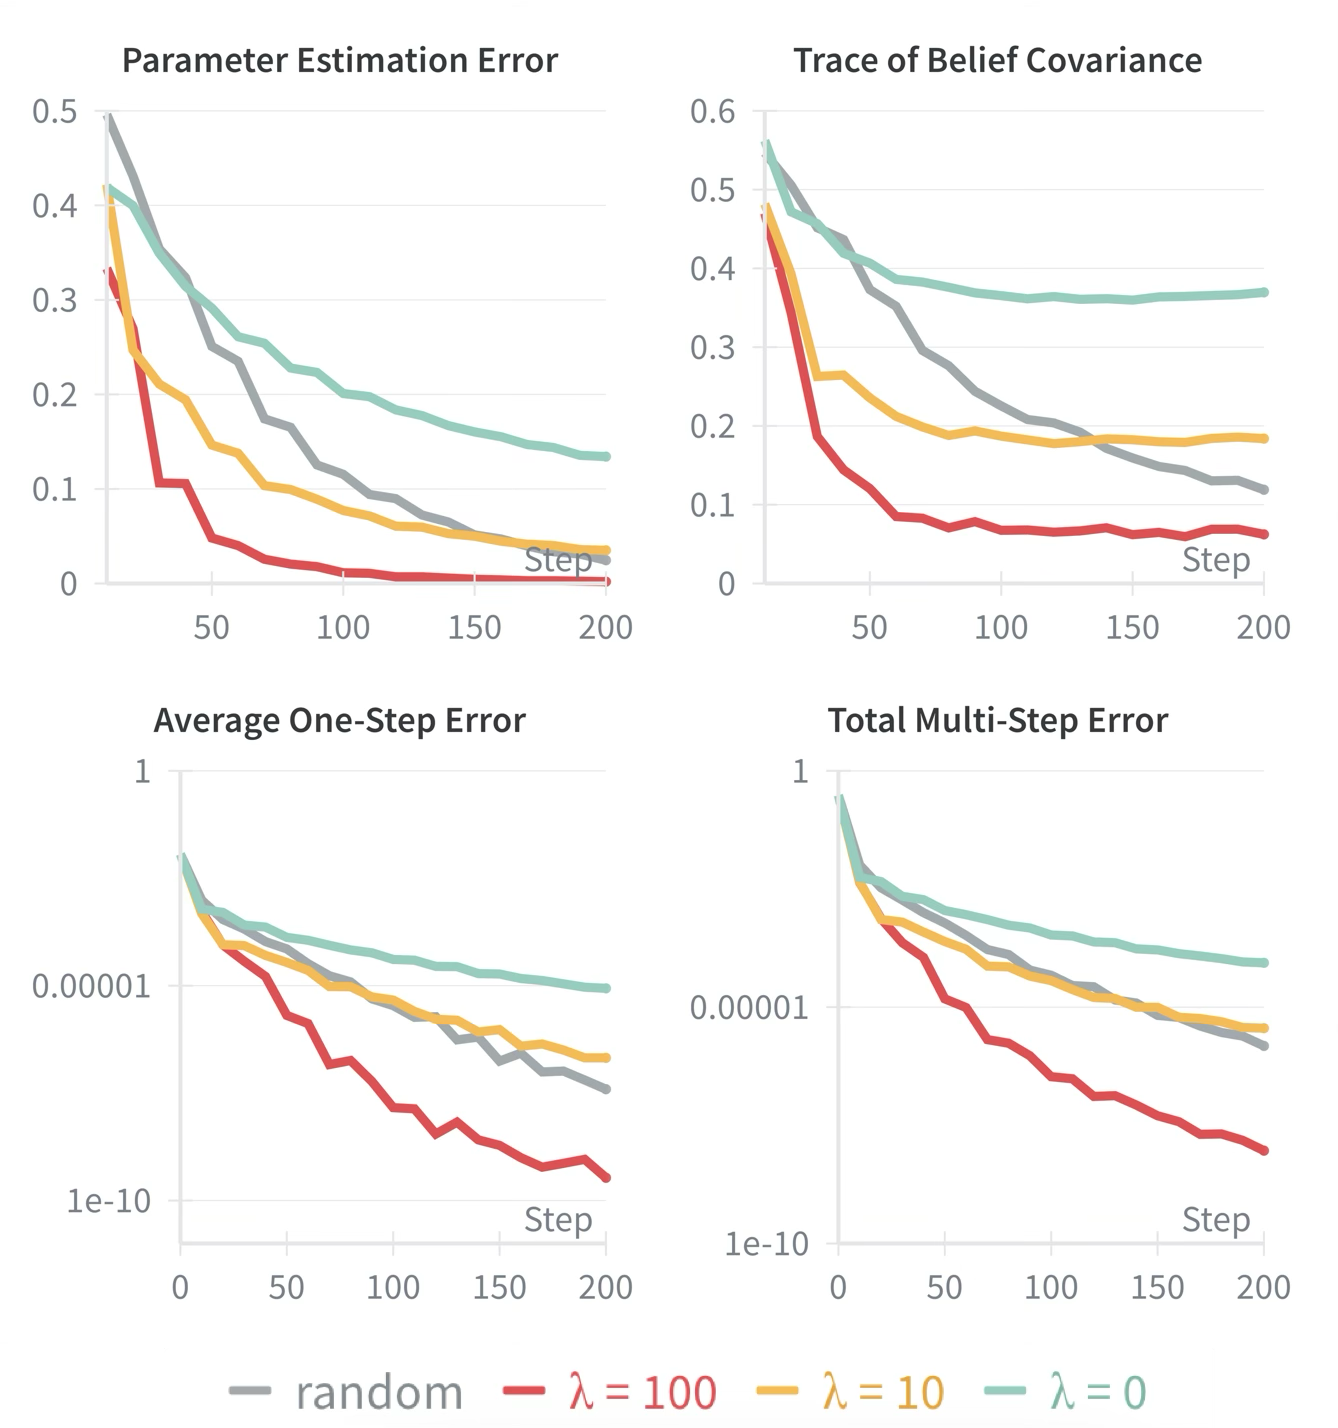
\includegraphics[width=\linewidth]{figures/pendulum.png}
\caption{Damped pendulum}
\label{fig:results_pendulum}
\end{minipage}
\end{minipage}

\vspace{1pt} % Space between rows

% Second row
\begin{minipage}{\linewidth}
\begin{minipage}{0.48\linewidth}
\centering
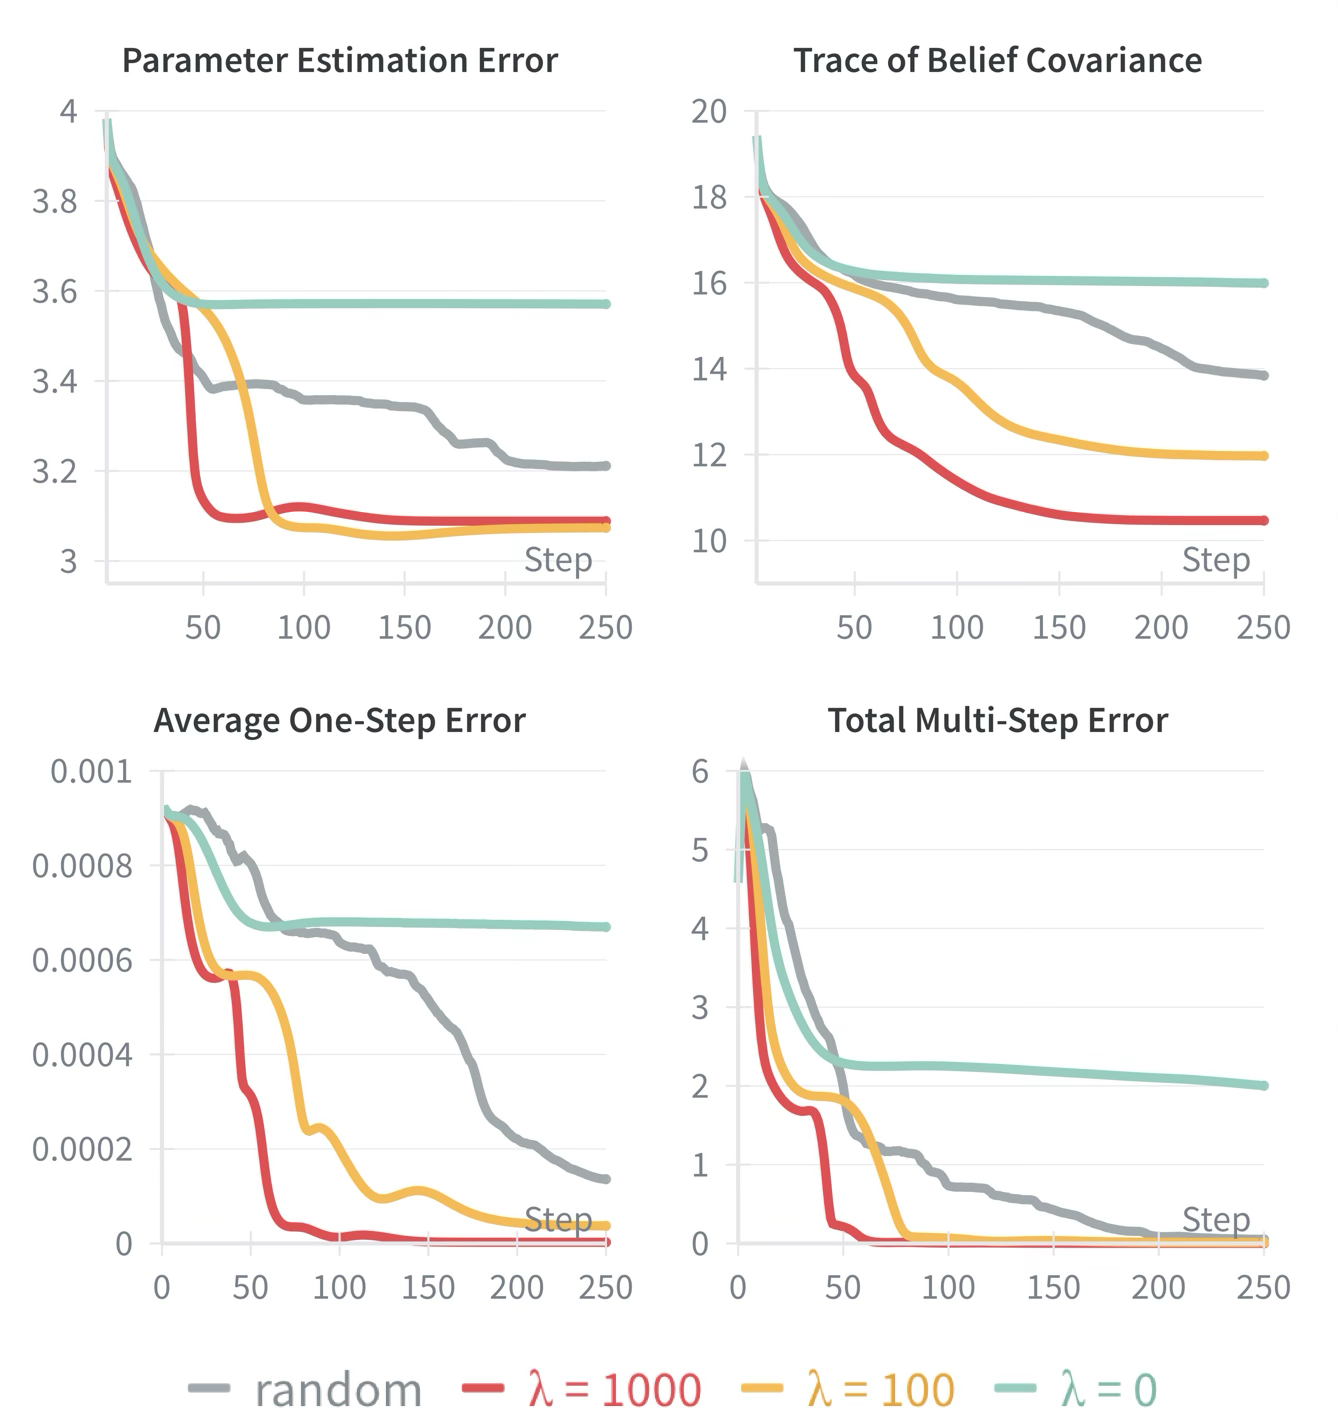
\includegraphics[width=\linewidth]{figures/lqr.png}
\caption{PE with LQR policy}
\label{fig:results_lqr}
\end{minipage}
\hfill
\begin{minipage}{0.48\linewidth}
\centering
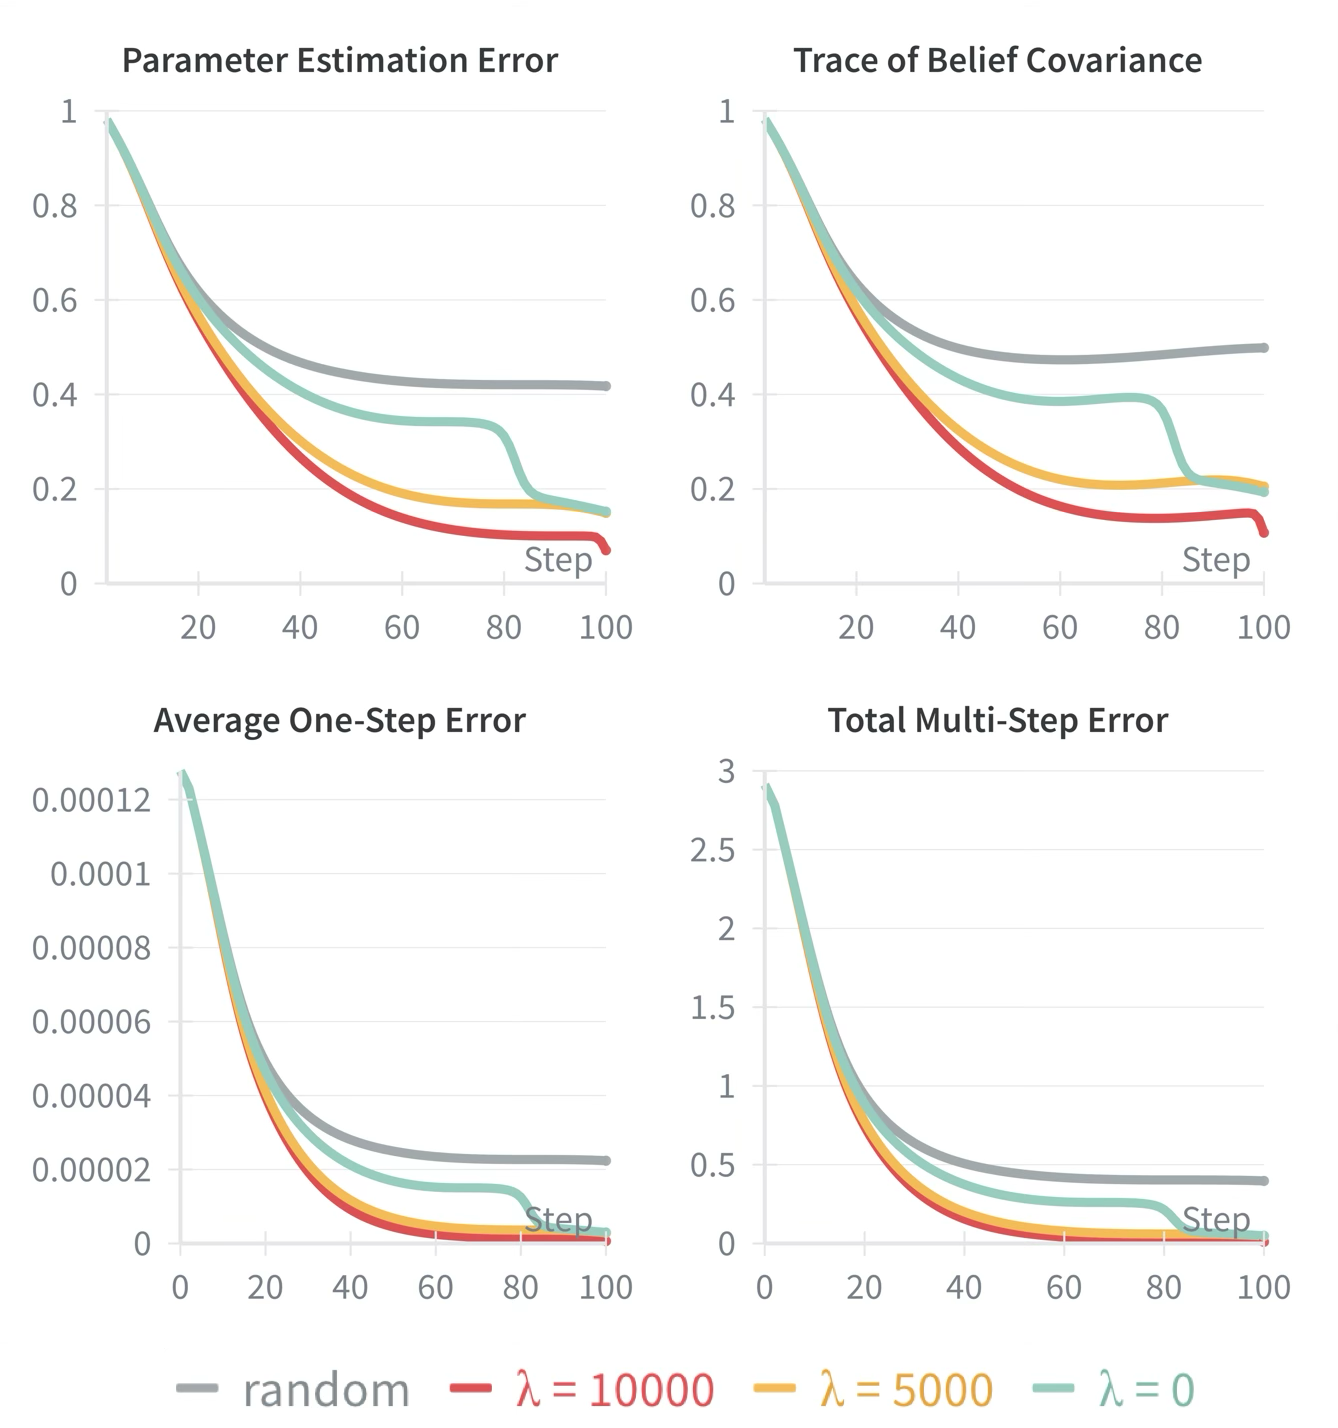
\includegraphics[width=\linewidth]{figures/unicycle.png}
\caption{PE with differentiable MPC}
\label{fig:results_unicycle}
\end{minipage}
\end{minipage}
\vspace{-30pt}
\end{figure}

% {\small
\textbf{Experiment 1: Single-agent linear system.} 
We consider an intentionally simplified setting in which a single agent operates under planar double integrator dynamics. The state is $\state_\timeindex = [p_x, p_y, v_x, v_y]^\top$ (position and velocity in 2D) and the control is $\control_\timeindex = [a_x, a_y]^\top$ (acceleration). The dynamics are $\state_{\timeindex+1} = \paramsA \state_{\timeindex} + \paramsB \control_{\timeindex}$ with unknown matrices $\paramsA \in \mathbb{R}^{4 \times 4}$ and $\paramsB \in \mathbb{R}^{4 \times 2}$. The task cost penalizes deviation from a goal state. Results are shown in \cref{fig:results_linear}.

\textbf{Experiment 2: Single-agent damped pendulum.} 
We consider a setting with more sophisticated nonlinear dynamics, in which a single agent controls a damped pendulum. The state is $\state_\timeindex = [\phi_\timeindex, \dot{\phi}_\timeindex]^\top$ (angle and angular velocity) and the control is $\control_\timeindex \in \mathbb{R}$ (applied torque). The dynamics are
\begin{equation*}
    \state_{\timeindex+1} = \begin{bmatrix}
        \phi_\timeindex + \dot{\phi}_\timeindex \Delta t \\
        \dot{\phi}_\timeindex + \ddot{\phi} \Delta t
    \end{bmatrix}
\end{equation*}
where $\ddot{\phi} = (\control_\timeindex - b\dot{\phi}_\timeindex - mgl\sin(\phi_\timeindex))/L$, with unknown damping coefficient $b$ and moment of inertia $L$. The task cost penalizes error in tracking a given reference angle. Results are shown in \cref{fig:results_pendulum}.

\textbf{Experiment 3: Two-agent pursuit-evasion with pursuer LQR policy.} 
We model a two-agent planar pursuit-evasion (PE) game where the pursuer follows an LQR policy with unknown cost matrices. Both agents have double integrator dynamics with states $\state_\timeindex^1, \state_\timeindex^2 \in \mathbb{R}^4$ (evader and pursuer positions/velocities) and controls $\control_\timeindex^1, \control_\timeindex^2 \in \mathbb{R}^2$ (accelerations). The full dynamics are
\begin{equation*}
    \state_{\timeindex+1} = \begin{bmatrix}
        \paramsA \state^1_\timeindex + \paramsB \control^1_\timeindex \\
        \paramsA \state^2_\timeindex + \paramsB \policy^2_\timeindex
    \end{bmatrix}
\end{equation*}
where the pursuer policy is $\policy^2_\timeindex = -(\paramsR + \paramsB^\top \paramsQ \paramsB)^{-1} \paramsB^\top \paramsQ (\paramsA \state^2_\timeindex - \state^1_\timeindex)$ with unknown (to agent 1) cost matrices $\paramsQ \in \mathbb{R}^{4 \times 4}$ and $\paramsR \in \mathbb{R}^{2 \times 2}$. The evader's task cost maximizes distance from the pursuer. Since dynamics for both agents are linear and assumed to be known, we can compute a closed-form LQR policy for the pursuer. Results are shown in \cref{fig:results_lqr}.

\textbf{Experiment 4: Two-agent pursuit-evasion with differentiable MPC policy.}
We extend the pursuit-evasion scenario to a pursuer with nonlinear unicycle dynamics. 
The evader maintains double integrator dynamics ($\state^1_\timeindex \in \mathbb{R}^4$, $\control^1_\timeindex \in \mathbb{R}^2$), while the pursuer has unicycle dynamics with state $\state^{\timeindex\top} = [p_{x,i}^2, p_{y,i}^2, \phi_i^2, v_i^2]$ (position, heading, speed) and control $\control^2_\timeindex = [\omega^2_i, a_i^2]^\top$ (angular velocity, acceleration). 
The pursuer dynamics are:
\begin{equation*}
    \state^2_{\timeindex+1} = \begin{bmatrix} 
        p_{x,\timeindex}^2 +  v_\timeindex^2 \cos(\phi_\timeindex^2)\Delta t \\ 
        p_{y,\timeindex}^2 +  v_\timeindex^2 \sin(\phi_\timeindex^2)\Delta t \\
        \phi_\timeindex^2 +  \omega_\timeindex^2 \Delta t\\
        v_\timeindex^2 +  a_\timeindex^2 \Delta t
    \end{bmatrix}
\end{equation*}
The pursuer policy is encoded by a nonlinear model predictive control problem with a cost parameter $w$ (unknown to the evader): $\policy^2_\timeindex = \arg\min_{\mathbf{u}} w\sum_{i=\timestart+1}^{\timestart + \horizon_\policy}\|\state^1_\timestart - \state^2_i\|^2 + \|\control_i\|^2$, implemented via differentiable optimization in \texttt{JAX} \cite{bradbury2018jax}. This experiment highlights how our framework can extend to a broad class of unknown dynamical models, including those with embedded optimization problems and games \cite{agrawal2019differentiable, amos2017optnet, blondel2022efficient, JMLR:TorchOpt, liu2023learning, liu2024auto, palafox2024smooth}. Results are shown in \cref{fig:results_unicycle}.
% }


% \begin{figure}[h!]
% \centering
% % First row
% \begin{minipage}{\linewidth}
% \begin{minipage}{0.48\linewidth}
% \centering
% 
\includegraphics[width=\linewidth]{figures/linear.png}
% \caption{Double integrator}
% \label{fig:results_linear}
% \end{minipage}
% \hfill
% \begin{minipage}{0.48\linewidth}
% \centering
% 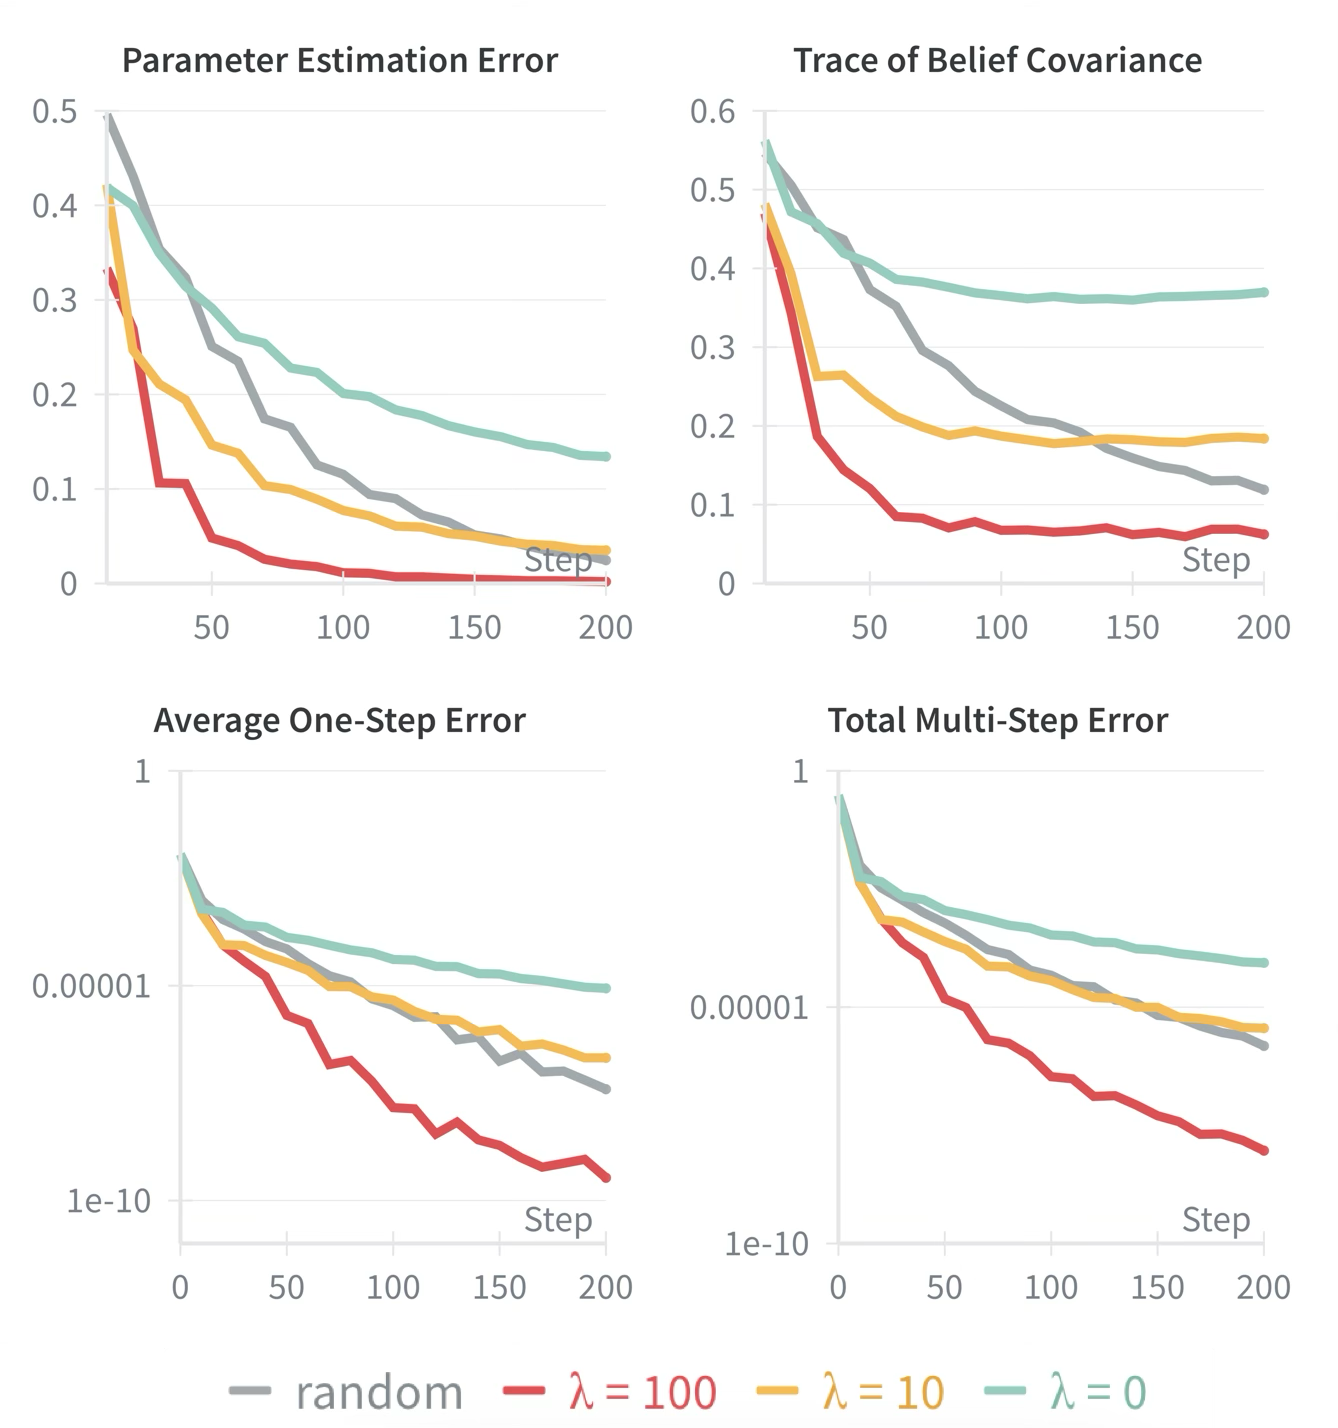
\includegraphics[width=\linewidth]{figures/pendulum.png}
% \caption{Damped pendulum}
% \label{fig:results_pendulum}
% \end{minipage}
% \end{minipage}

% \vspace{1pt} % Space between rows

% % Second row
% \begin{minipage}{\linewidth}
% \begin{minipage}{0.48\linewidth}
% \centering
% 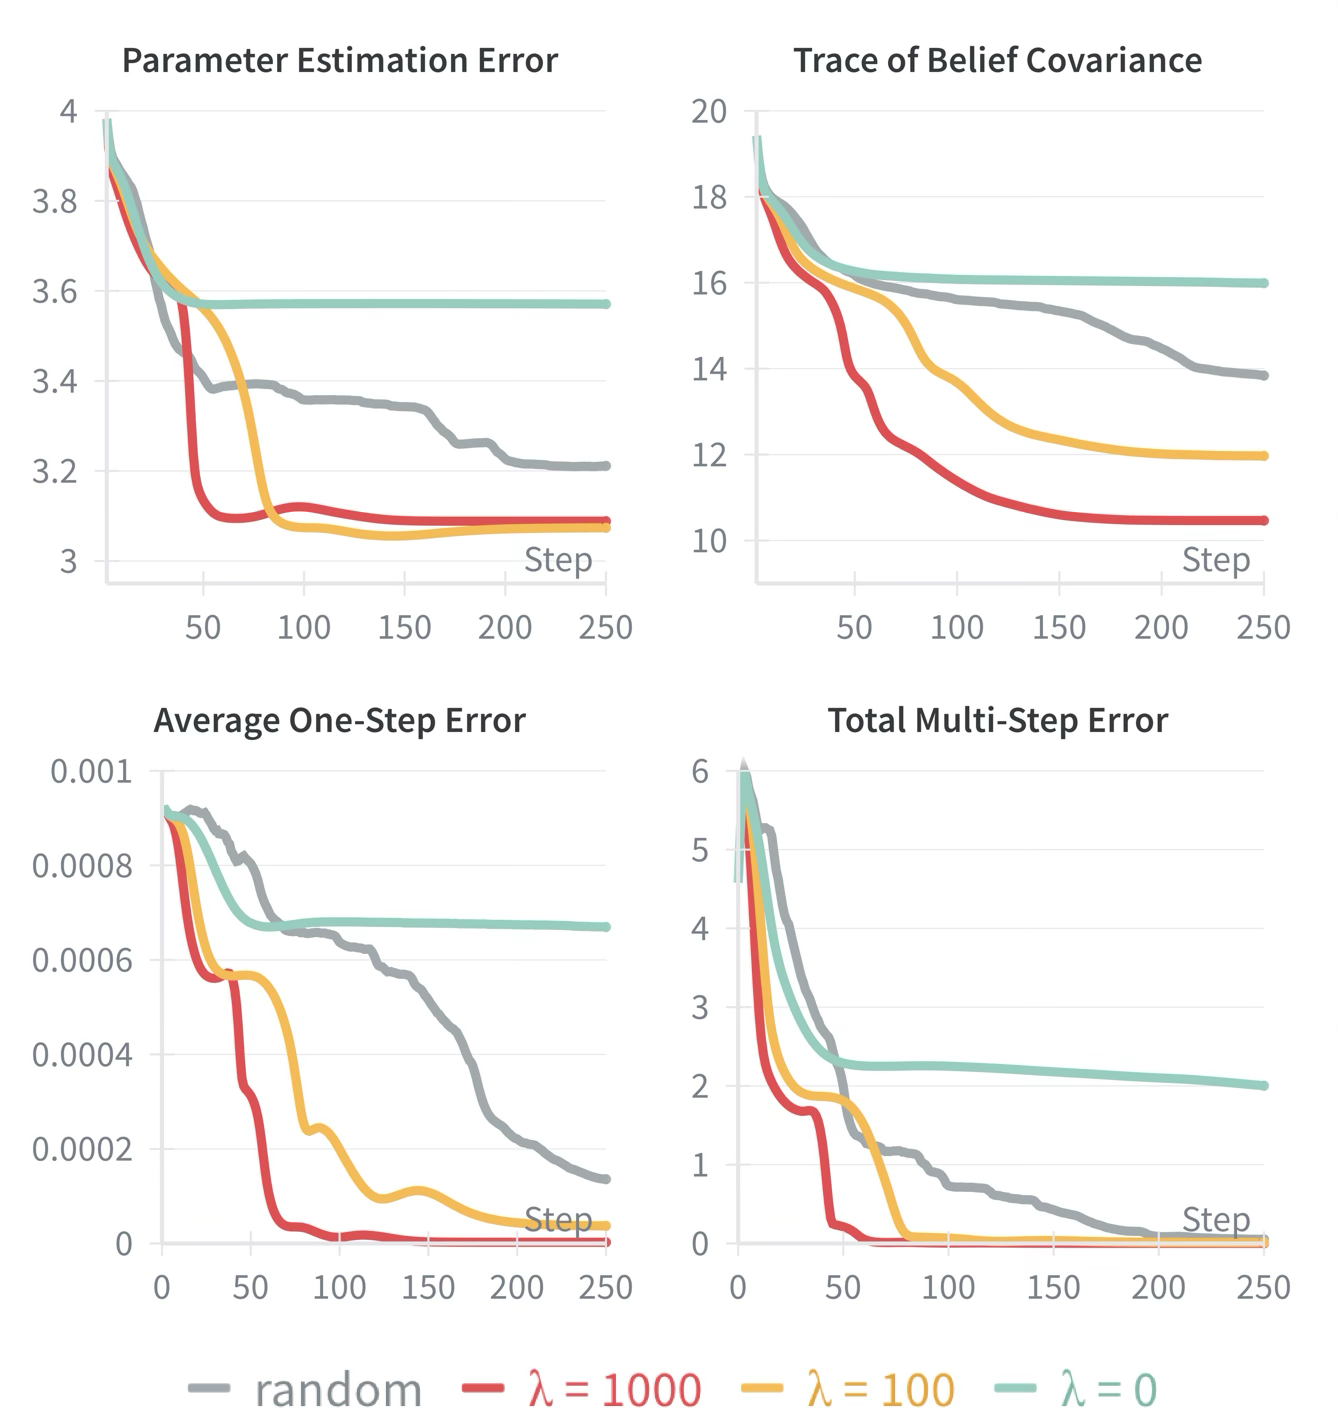
\includegraphics[width=\linewidth]{figures/lqr.png}
% \caption{PE with LQR policy}
% \label{fig:results_lqr}
% \end{minipage}
% \hfill
% \begin{minipage}{0.48\linewidth}
% \centering
% \includegraphics[width=\linewidth]{figures/uni.png}
% \caption{PE with differentiable MPC}
% \label{fig:results_unicycle}
% \end{minipage}
% \end{minipage}
% \vspace{-10pt}
% \end{figure}

% \subsection{Experimental Results}

% \begin{figure}[h]
% \centering
% \begin{minipage}{0.48\linewidth}
% \centering
% \includegraphics[width=\linewidth]{figures/results_linear.png}
% \caption{Single-agent linear system}
% \label{fig:results_linear}
% \end{minipage}
% \hfill
% \begin{minipage}{0.48\linewidth}
% \centering
% \includegraphics[width=\linewidth]{figures/results_pendulum.png}
% \caption{Single-agent damped pendulum}
% \label{fig:results_pendulum}
% \end{minipage}
% \end{figure}

% \begin{figure}[h]
% \centering
% \begin{minipage}{0.48\linewidth}
% \centering
% \includegraphics[width=\linewidth]{figures/results_lqr.png}
% \caption{Two-agent pursuit-evasion with pursuer LQR}
% \label{fig:results_lqr}
% \end{minipage}
% \hfill
% \begin{minipage}{0.48\linewidth}
% \centering
% \includegraphics[width=\linewidth]{figures/results_unicycle.png}
% \caption{Two-agent pursuit-evasion with differentiable pursuer policy}
% \label{fig:results_unicycle}
% \end{minipage}
% \end{figure}



\subsection{Discussion}
Across all experiments in \cref{fig:results_linear,fig:results_pendulum,fig:results_lqr,fig:results_unicycle}, increasing the information-gathering weight $\lambda$ (yellow and red lines) reduces parameter estimation error and improves generalization to held-out data, compared to the random and passive learning baselines.
We remark that in Experiment 4 (\cref{fig:results_unicycle}), the passive learning trajectory ($\lambda = 0$) performs better than the random baseline. 
We conjecture this is because, in certain settings, local minima for the task and information-gathering costs lie in the same regions of state space. 
Therefore, passive learning results in enough excitation for accurate parameter identification.

The results confirm both of our hypotheses: active information gathering accelerates parameter learning and improves model generalization compared to passive observation.
The experiments also validate the claim in \cref{sec:contribution3} that the mutual information cost from \Cref{thm:mi_special_case} directly accelerates parameter learning.
Finally, they showcase how our framework applies across single-agent and multi-agent problems with both linear and nonlinear dynamics.

% The improved generalization likely arises because active information gathering drives the agent toward areas with richer information content, yielding models that extrapolate better to unseen transitions.
Our framework's modularity enabled rapid instantiation of these diverse experiments: we applied the same EKF belief updater and mutual information cost with linear dynamics, nonlinear dynamics, and embedded differentiable model predictive control modules encoding unknown opponent behavior, all without any problem-specific cost derivations.
This validates the practical utility of our formalization beyond theoretical generality.

\contribution[Experimental validation in single and multi-agent settings.]{
Our experiments showcase the practical utility of our framework by demonstrating information-gathering behavior in a variety of dynamical systems (single-agent, multi-agent, linear, non-linear) without problem-specific cost derivations.}

